% !TEX root=talk.tex

\section{Document Types}

\begin{frame}[fragile,allowframebreaks]
\frametitle{Basic Types}
\begin{columns}
\begin{column}{.35\textwidth}
\begin{beamerboxesrounded}[width=\linewidth]{Books}
\begin{lstlisting}[moretexcs={chapter,subsection,maketitle}, basicstyle={\ttfamily}, emph={book}]
\documentclass{book}
\author{...}
\title{...}

\begin{document}
\maketitle
\chapter{...}
\section{...}
...
\subsection{...}
\end{document}
\end{lstlisting}
\end{beamerboxesrounded}
\end{column}
\begin{column}{.58\textwidth}
\centering
\fcolorbox{black}{white}{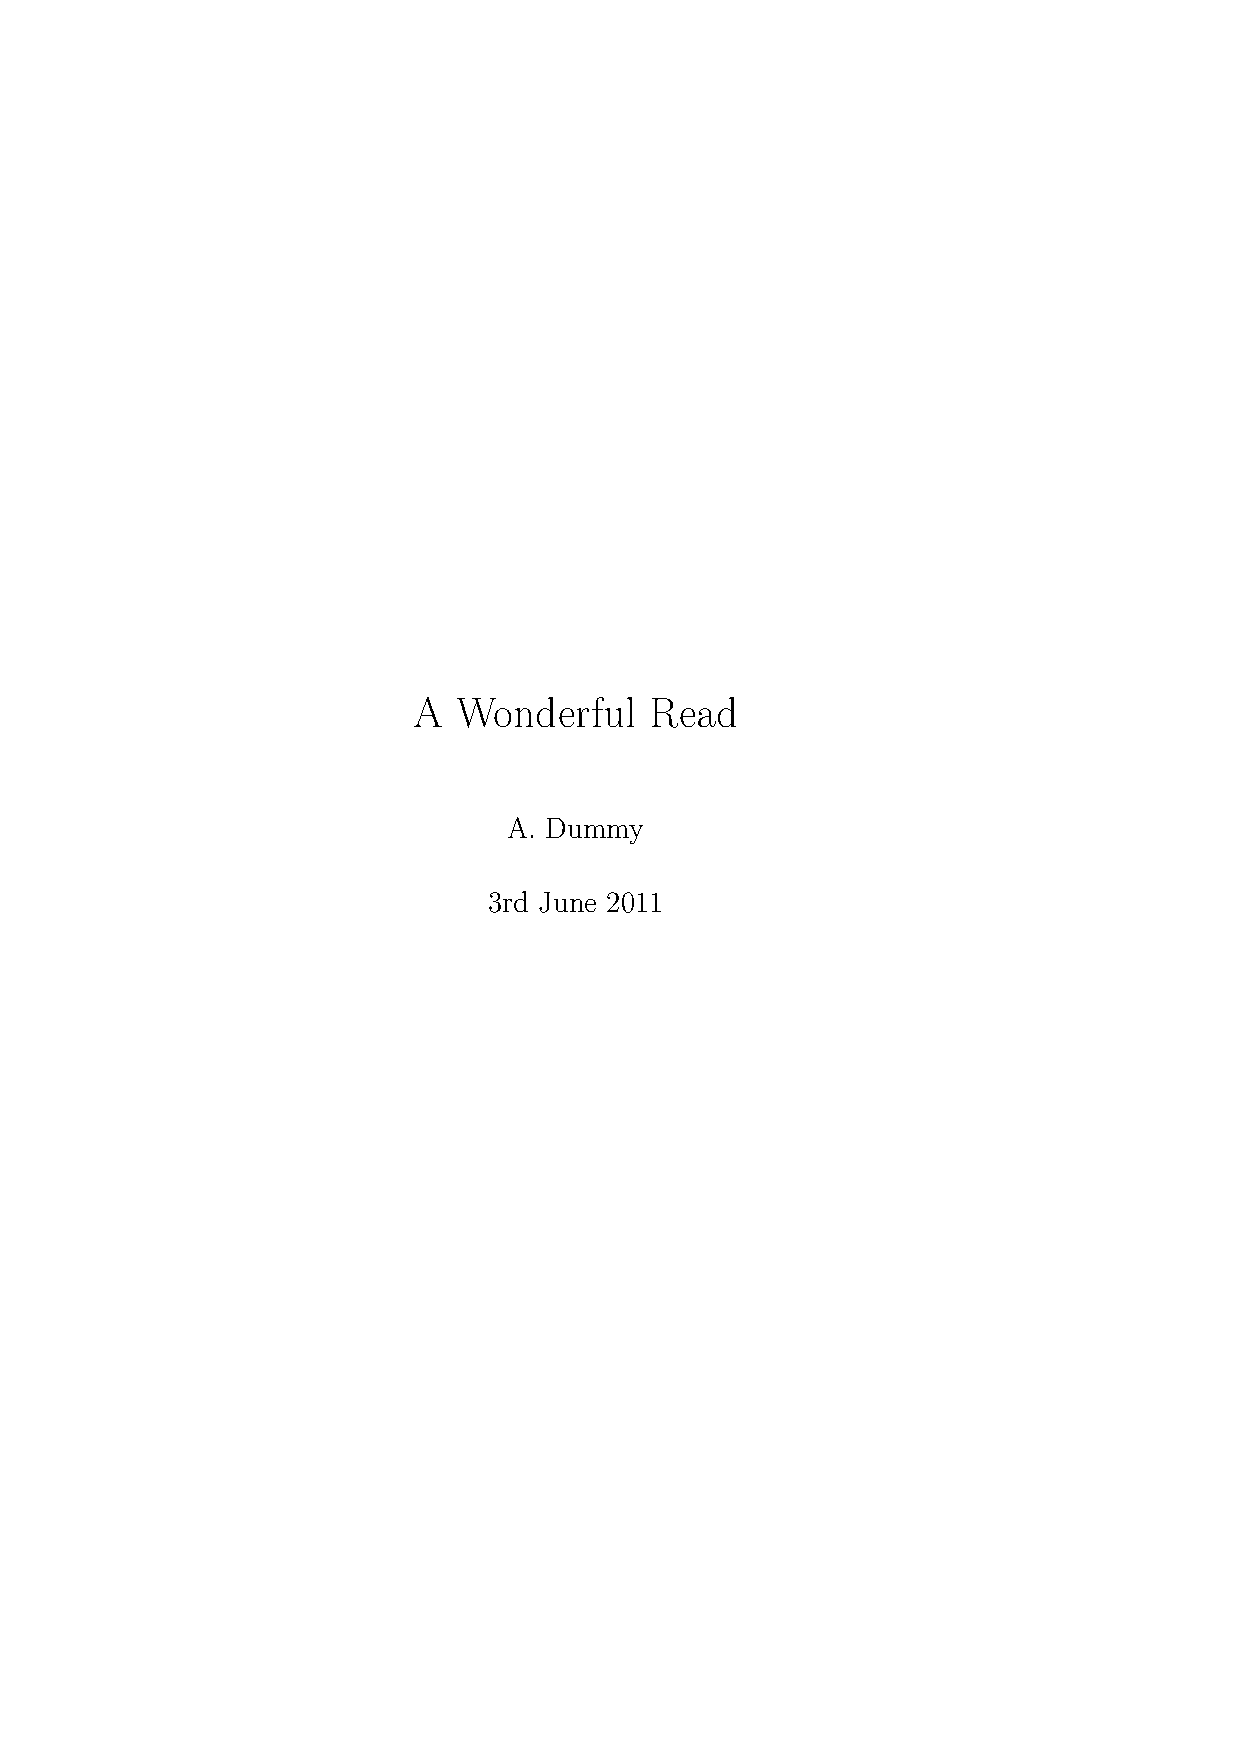
\includegraphics[width=.4\linewidth,page=1]{examples/basicbook}}
\fcolorbox{black}{white}{\includegraphics[width=.4\linewidth,page=3]{examples/basicbook}}
\fcolorbox{black}{white}{\includegraphics[width=.4\linewidth,page=4]{examples/basicbook}}
\fcolorbox{black}{white}{\includegraphics[width=.4\linewidth,page=5]{examples/basicbook}}
\end{column}
\end{columns}

\begin{columns}
\begin{column}{.4\textwidth}
\begin{beamerboxesrounded}[width=\linewidth]{Articles}
\begin{lstlisting}[moretexcs={chapter,subsection,maketitle}, basicstyle={\ttfamily}, emph={article}]
\documentclass{article}
\author{...}
\title{...}

\begin{document}
\maketitle
\section{...}
...
\subsection{...}
\end{document}
\end{lstlisting}
\end{beamerboxesrounded}
\end{column}
\begin{column}{.58\textwidth}
\centering
\fcolorbox{black}{white}{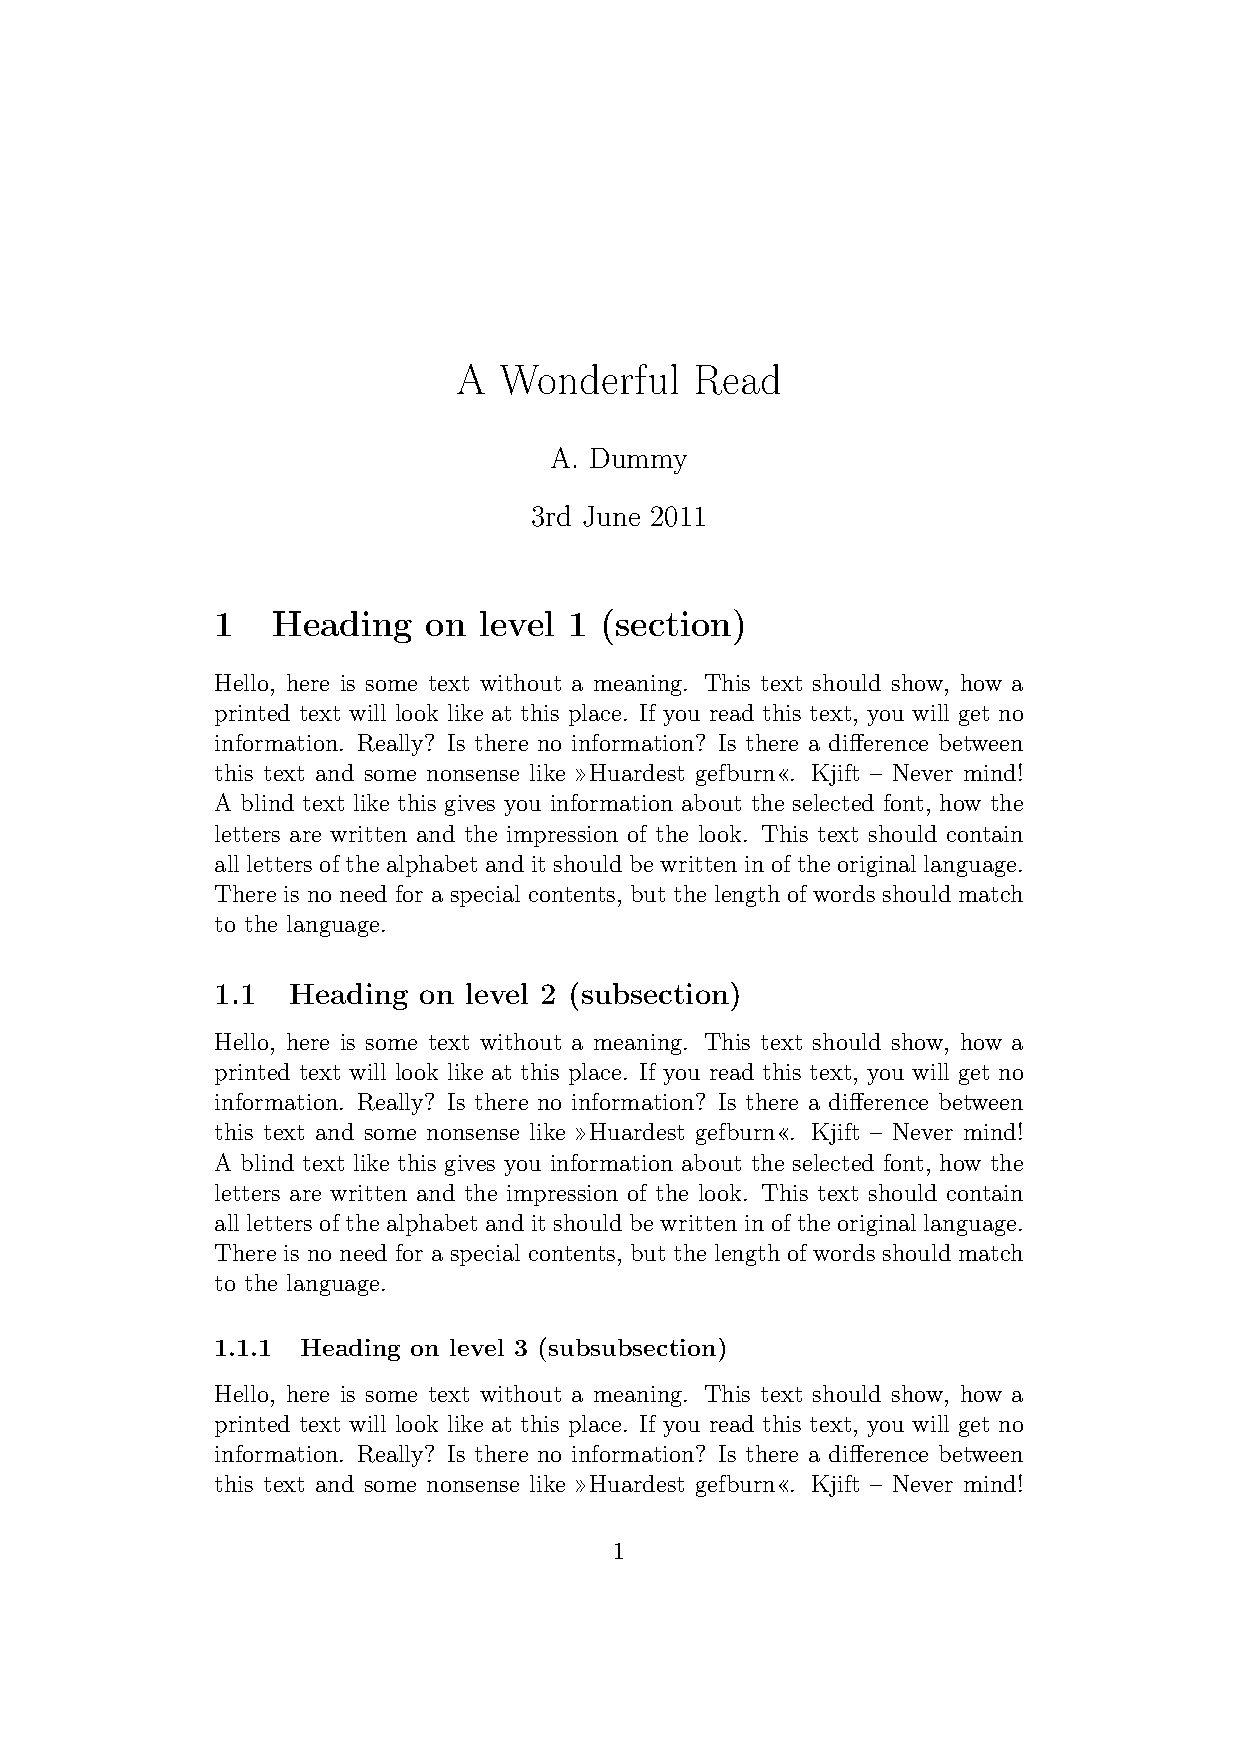
\includegraphics[width=.4\linewidth,page=1]{examples/basicarticle}}
\fcolorbox{black}{white}{\includegraphics[width=.4\linewidth,page=2]{examples/basicarticle}}
\fcolorbox{black}{white}{\includegraphics[width=.4\linewidth,page=3]{examples/basicarticle}}
\fcolorbox{black}{white}{\includegraphics[width=.4\linewidth,page=4]{examples/basicarticle}}
\end{column}
\end{columns}
\end{frame}

\begin{frame}[fragile]
\frametitle{Journal and Conference Proceedings Articles}
\begin{columns}[T]
\begin{column}{.33\textwidth}
\textsmaller{IEEE}\\\lstinline[basicstyle=\ttfamily\small]|\documentclass{IEEEtran}|
\vskip.5em
\fcolorbox{black}{white}{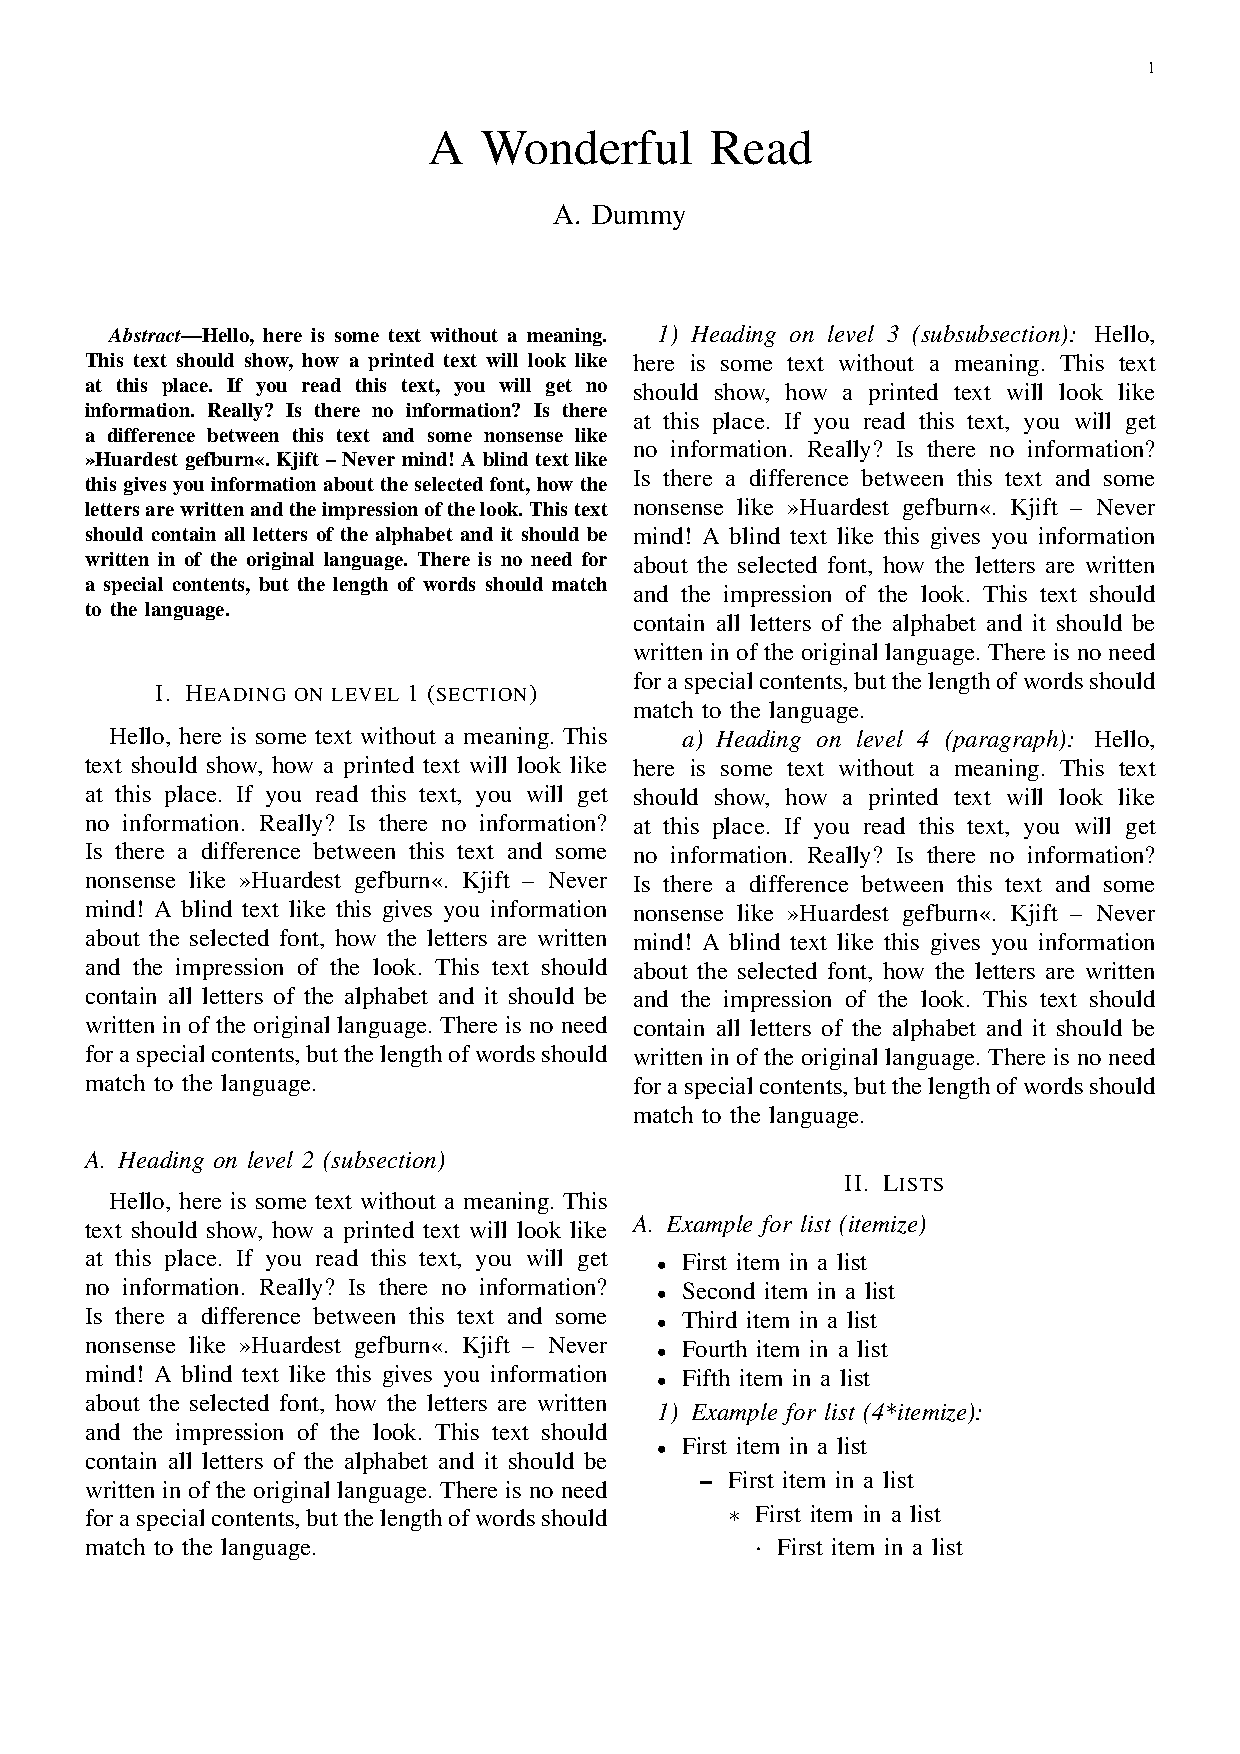
\includegraphics[width=\linewidth,page=1]{examples/IEEEtran}}
\end{column}

\begin{column}{.33\textwidth}
\textsmaller{ACM}\\\lstinline[basicstyle=\ttfamily\footnotesize\lsstyle,emphstyle=\scriptsize]|\documentclass{sig-alternate}|
\vskip.5em
\fcolorbox{black}{white}{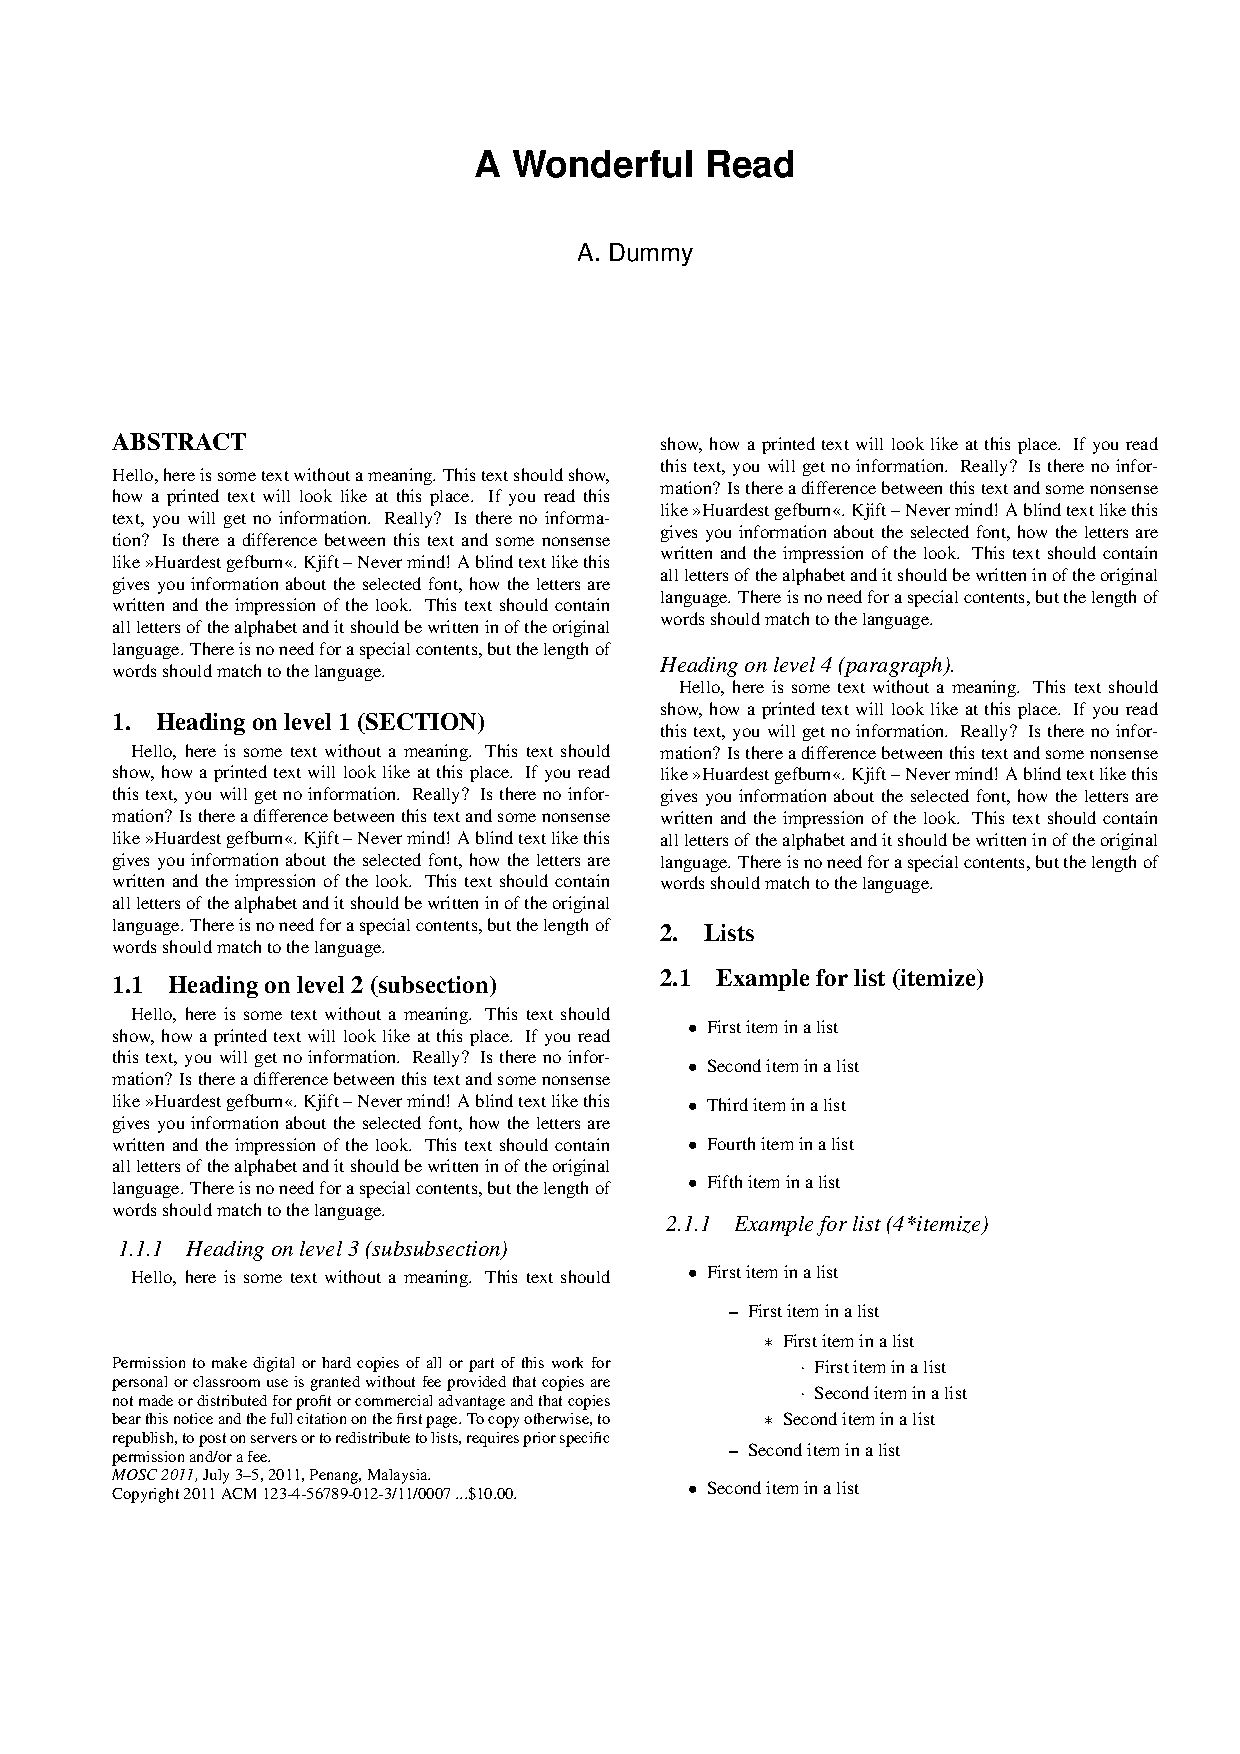
\includegraphics[width=\linewidth,page=1]{examples/acmconf}}
\end{column}

\begin{column}{.33\textwidth}
\textsmaller{LLNCS}\\\lstinline[basicstyle=\ttfamily\small]|\documentclass{llncs}|
\vskip.5em
\fcolorbox{black}{white}{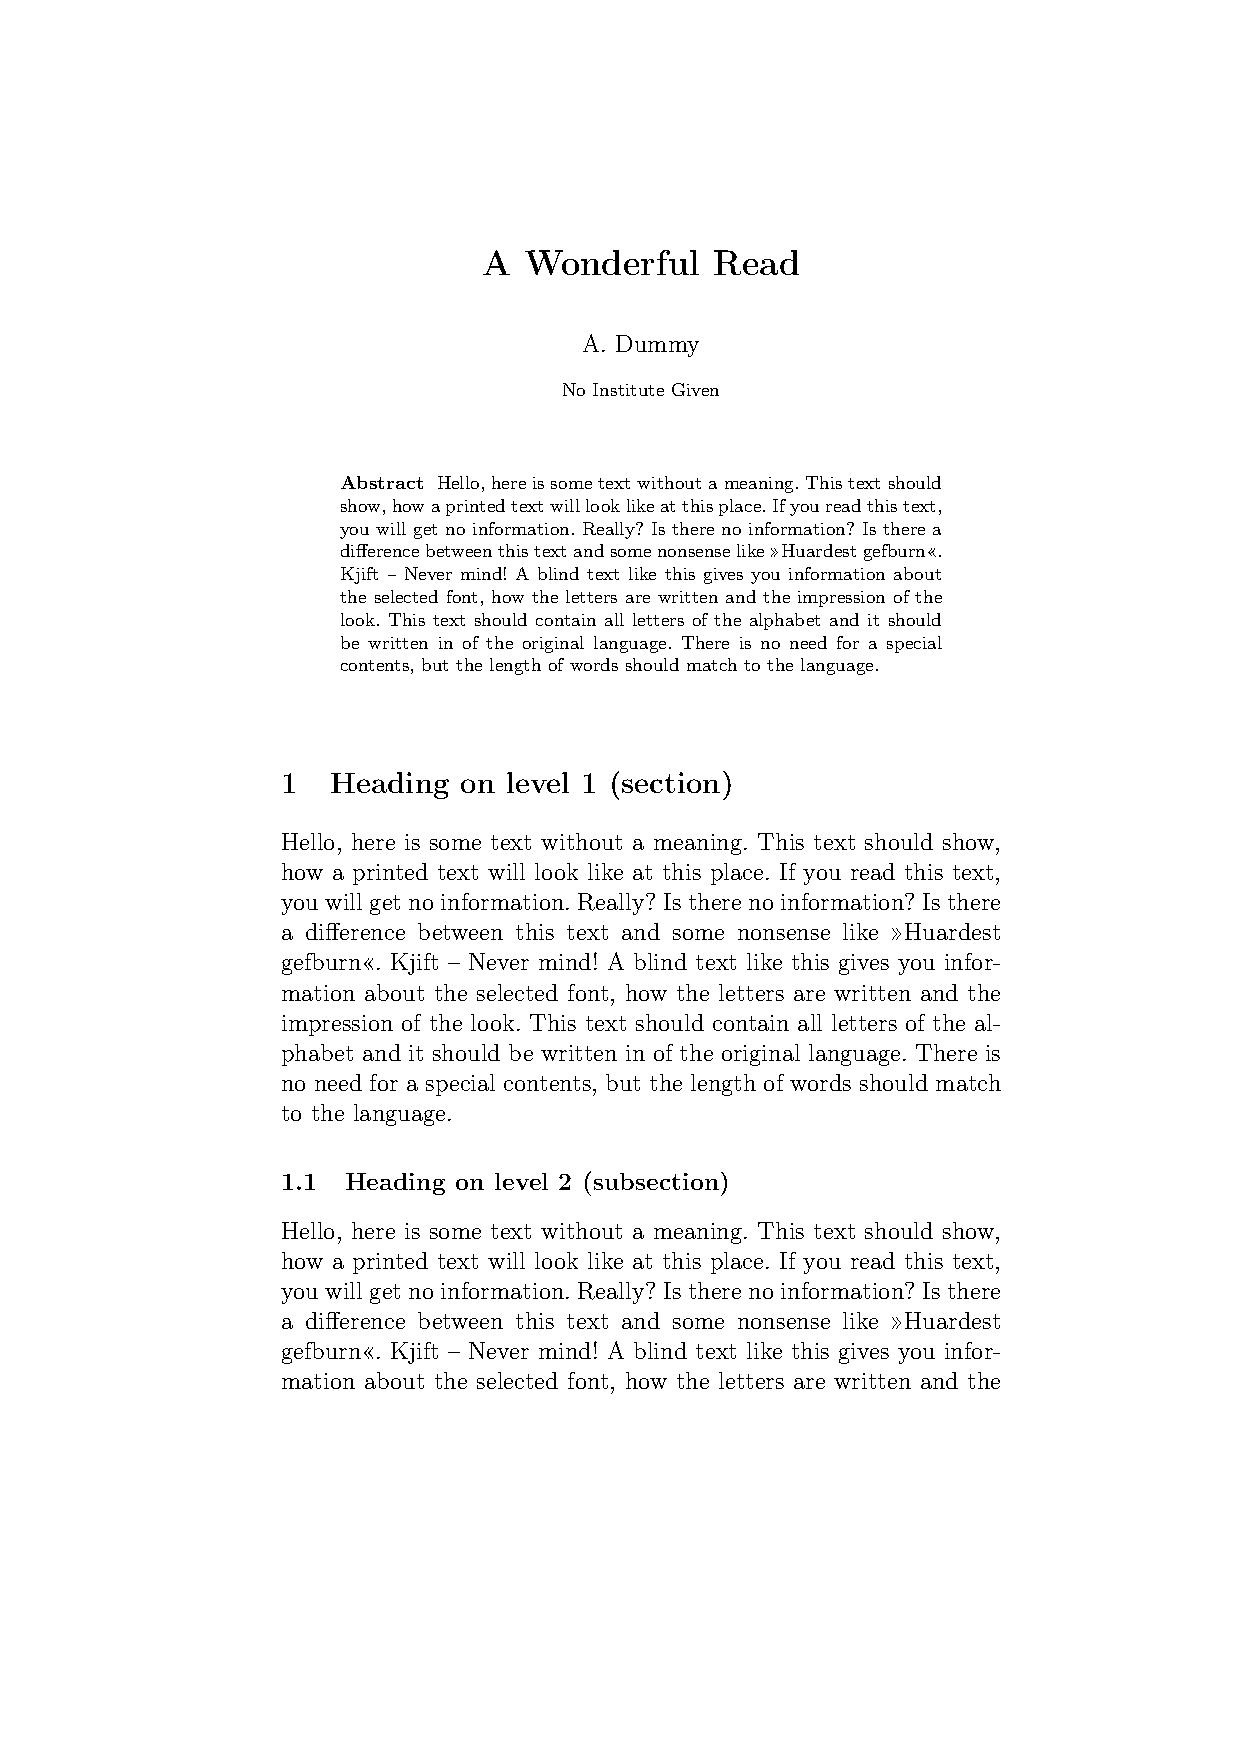
\includegraphics[width=\linewidth,page=1]{examples/llncs}}
\end{column}
\end{columns}
\end{frame}


\begin{frame}[fragile]
\lstset{basicstyle=\ttfamily}
\frametitle{Some Goodies}
\begin{itemize}
\item<+> Quick \structure{language-switching} with \texttt{babel}
\item<+> Automatic generation of \structure{cross-referencing labels}:\\
\lstinline|\section{Introduction}\label{sec:intro}|\\
\lstinline|... We saw in section \ref{sec:intro}...|
\item<+> Automatic generation of \structure{lists}:\\
\lstinline[texcs={tableofcontents}]|\tableofcontents|, \lstinline[texcs={listoffigures}]|\listoffigures|,  \lstinline[texcs={listoftables}]|\listoftables|
\item<+> Automatic generation of \structure{bibliographies} and \structure{indices}:\\
\lstinline|\cite{Knuth:1976}...\bibliography{references.bib}|\\
\lstinline[moretexcs={printindex}]|...the Linux kernel\index{Linux!kernel}... \printindex|\\
\item<+> Fully \structure{hyperlinked} \textsmaller{PDF} with bookmarks: \lstinline|\usepackage{hyperref}|
\item<+> Inclusion of selected pages from other \textsmaller{PDF}s\\(while inserting new page headers/footers!)\\
\lstset{basicstyle=\ttfamily\footnotesize,moretexcs={includepdf}}
\lstinline|\usepackage{pdfpages}|\\
\lstinline|\includepdf[pages={1,3-5,8},pagecommand=\thispagestyle{plain}]{file.pdf}|
\end{itemize}
\end{frame}

\begin{frame}
\frametitle{Multilingual \hologo{LaTeX}}
\centering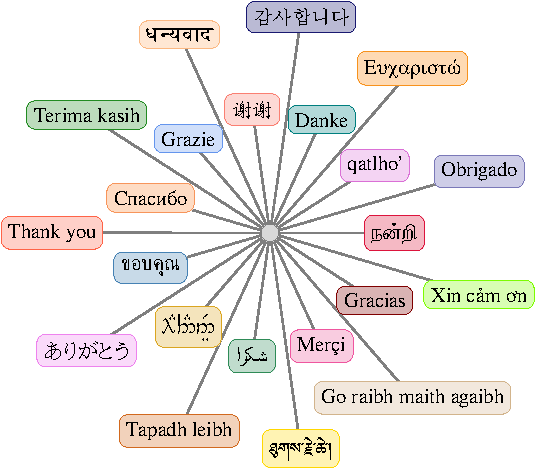
\includegraphics[height=.7\textheight]{multiling-TQ}\par
\pause
\begin{description}
\item[\hologo{XeLaTeX}, \hologo{LuaLaTeX}] Unicode input
\item[\hologo{LaTeX}] Various packages {\small (sometimes with transcriptions:  \texttt{nan\textasciicircum ri}, \texttt{salAm})}
\end{description}
\end{frame}

\begin{frame}[fragile,allowframebreaks]
\frametitle{University Theses}
\small
Universiti Sains Malaysia \lstinline[basicstyle=\ttfamily]|\documentclass{usmthesis}|
\vskip.5em

%% See http://liantze.penguinattack.org/latextypesetting.html#usmthesis
{\centering
\fcolorbox{black}{white}{
\includegraphics[width=.24\linewidth,page=2]{examples/usmthesis.pdf}}
\fcolorbox{black}{white}{
\includegraphics[width=.24\linewidth,page=4]{examples/usmthesis.pdf}}
\fcolorbox{black}{white}{
\includegraphics[width=.24\linewidth,page=13]{examples/usmthesis.pdf}}
\fcolorbox{black}{white}{
\includegraphics[width=.24\linewidth,page=36]{examples/usmthesis.pdf}}\par}

\mode<beamer>{
\pagebreak

%% See http://liantze.penguinattack.org/latextypesetting.html#mmuthesis
Multimedia University {\ttfamily{\color{Maroon}\bfseries\textbackslash documentclass}\{mmuthesis\}}
\vskip.5em

{\centering
\fcolorbox{black}{white}{
\includegraphics[width=.24\linewidth,page=3]{examples/mmuthesis.pdf}}
\fcolorbox{black}{white}{
\includegraphics[width=.24\linewidth,page=9]{examples/mmuthesis.pdf}}
\fcolorbox{black}{white}{
\includegraphics[width=.24\linewidth,page=13]{examples/mmuthesis.pdf}}
\fcolorbox{black}{white}{
\includegraphics[width=.24\linewidth,page=18]{examples/mmuthesis.pdf}}
\par}

\pagebreak

%% See http://liantze.penguinattack.org/latextypesetting.html#umalayathesis
Universiti Malaya {\ttfamily{\bfseries\color{Maroon}\textbackslash documentclass}\{umalayathesis\}}
\vskip.5em

{\centering
\fcolorbox{black}{white}{\includegraphics[width=.24\linewidth,page=2]{examples/umalayathesis.pdf}}
\fcolorbox{black}{white}{\includegraphics[width=.24\linewidth,page=6]{examples/umalayathesis.pdf}}
\fcolorbox{black}{white}{\includegraphics[width=.24\linewidth,page=12]{examples/umalayathesis.pdf}}
\fcolorbox{black}{white}{\includegraphics[width=.24\linewidth,page=20]{examples/umalayathesis.pdf}}
\par}}

\end{frame}


\begin{frame}
\frametitle{Highly Configurable Documents}
\framesubtitle{\texttt{memoir} and \textsmaller{KOMA}-Script Classes}

\begin{itemize}
\item Sectional headings
\item Running headers and footers
\item Good font, colour and illustration choices
\item \url{http://latex-my.blogspot.com/search/label/bookdesign}
\end{itemize}

%% See http://liantze.penguinattack.org/ebooks.html
\begin{center}
\onslide<2>{%
%\fcolorbox{black}{white}{\includegraphics[width=.24\linewidth,page=1]{examples/GridComputingCluster-Report2009}}
%\fcolorbox{black}{white}{\includegraphics[width=.24\linewidth,page=5]{examples/GridComputingCluster-Report2009}}
%\fcolorbox{black}{white}{\includegraphics[width=.24\linewidth,page=10]{examples/GridComputingCluster-Report2009}}
%\fcolorbox{black}{white}{\includegraphics[width=.24\linewidth,page=32]{examples/GridComputingCluster-Report2009}}
%}
\fcolorbox{black}{white}{
\includegraphics[width=.24\linewidth,page=1]{examples/GridBookExcerpt}}
\fcolorbox{black}{white}{
\includegraphics[width=.24\linewidth,page=2]{examples/GridBookExcerpt}}
\fcolorbox{black}{white}{
\includegraphics[width=.24\linewidth,page=3]{examples/GridBookExcerpt}}
\fcolorbox{black}{white}{
\includegraphics[width=.24\linewidth,page=4]{examples/GridBookExcerpt}}
}
\end{center}
\end{frame}



\begin{frame}[fragile]
\frametitle{Presentation Slides}
\begin{itemize}
\item This presentation was made with \LaTeX!
\item<+-> Many possible classes: \texttt{powerdot}, \alert<2->{\texttt{beamer}}
\end{itemize}

\begin{columns}<+->
\begin{column}{.47\textwidth}
\begin{beamerboxesrounded}[width=\linewidth]{}
\vskip-1em
\begin{lstlisting}[basicstyle=\ttfamily\small,
moretexcs={usetheme,frametitle,frame,titleframe},
emph={beamer,frame},
escapechar={:},lineskip=-2pt]
\documentclass{beamer}
\usetheme{:\onslide<2>{Warsaw}%
\onslide<3|trans:0|handout:0>{\llap{Szeged}}%
\onslide<4|trans:0|handout:0>{\llap{Bergen}}%
\onslide<5|trans:0|handout:0>{\llap{oxygen}}%
\onslide<6|trans:0|handout:0>{\llap{Gelugor}}:}

\author ...

\begin{document}
\titleframe

\section{Intro}

\begin{frame}
\frametitle{Some Background}
...
:\bfseries\color{Maroon}\textbackslash end:{frame}
\end{document}
\end{lstlisting}
\vspace*{-1em}
\end{beamerboxesrounded}
\end{column}
\begin{column}{.48\textwidth}
\centering
\onslide<2>{\fcolorbox{black}{white}{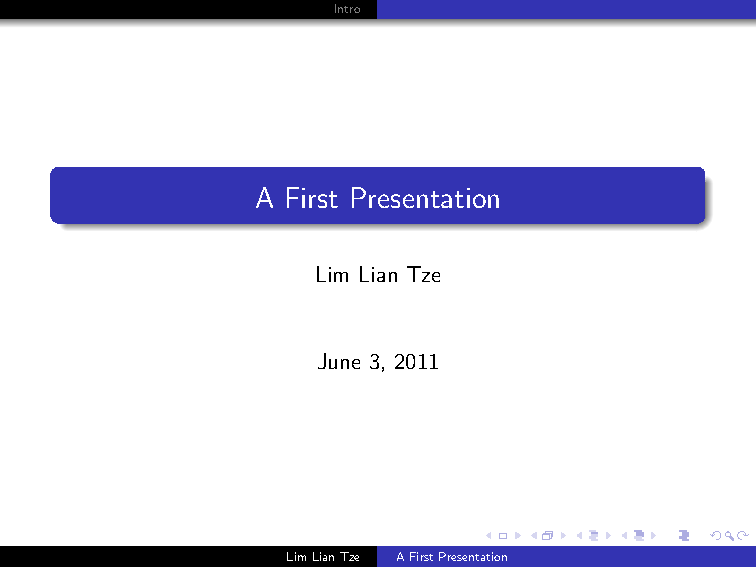
\includegraphics[width=.7\linewidth,page=1]{examples/beamer-Warsaw}}}%
\onslide<3|trans:0|handout:0>{\llap{\fcolorbox{black}{white}{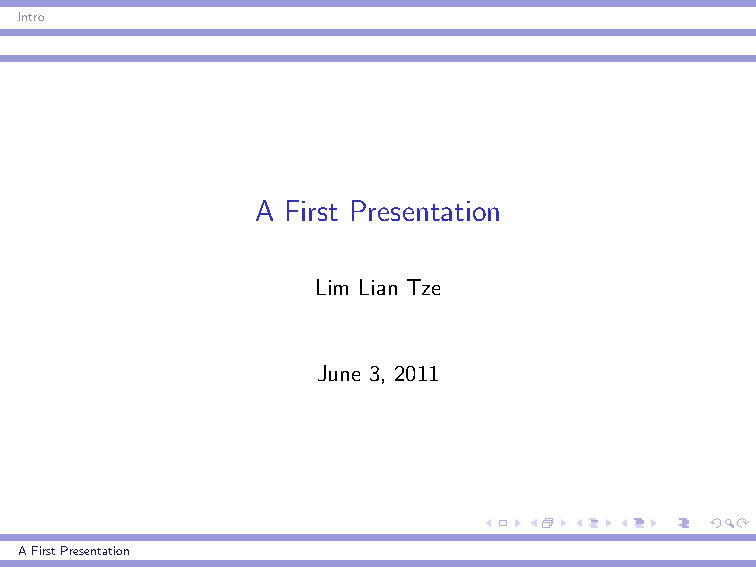
\includegraphics[width=.7\linewidth,page=1]{examples/beamer-Szeged}}
}}%
\onslide<4|trans:0|handout:0>{\llap{\fcolorbox{black}{white}{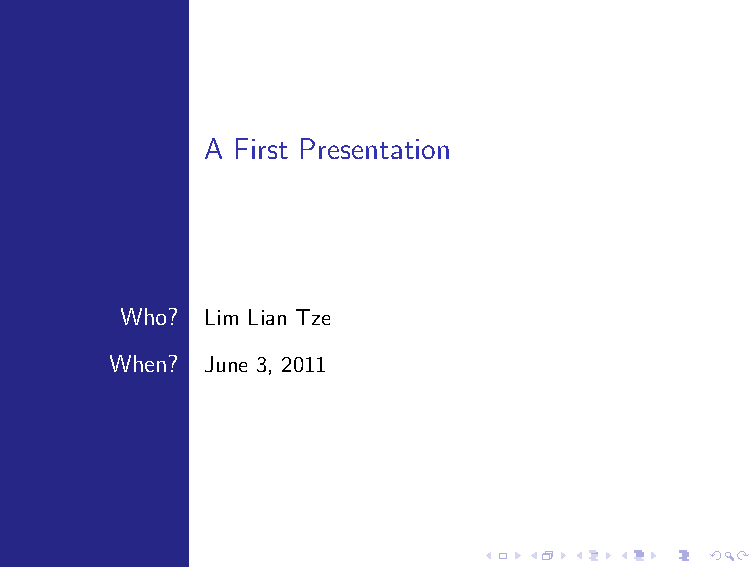
\includegraphics[width=.7\linewidth,page=1]{examples/beamer-Bergen}}
}}%
\onslide<5|trans:0|handout:0>{\llap{\fcolorbox{black}{white}{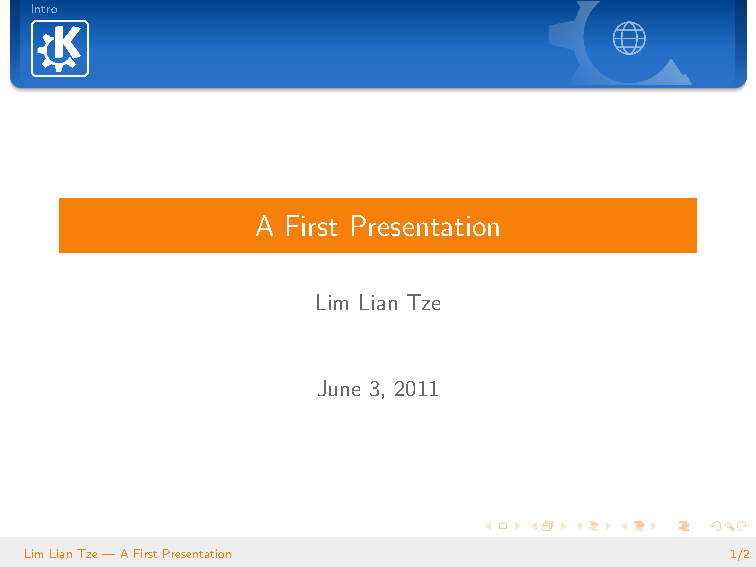
\includegraphics[width=.7\linewidth,page=1]{examples/beamer-Oxygen}}
}}%
\onslide<6|trans:0|handout:0>{\llap{\fcolorbox{black}{white}{
\includegraphics[width=.7\linewidth,page=1]{examples/beamer-Gelugor}}
}}
\onslide<2>{\fcolorbox{black}{white}{\includegraphics[width=.7\linewidth,page=2]{examples/beamer-Warsaw}}}%
\onslide<3|trans:0|handout:0>{\llap{\fcolorbox{black}{white}{\includegraphics[width=.7\linewidth,page=2]{examples/beamer-Szeged}}
}}%
\onslide<4|trans:0|handout:0>{\llap{\fcolorbox{black}{white}{\includegraphics[width=.7\linewidth,page=2]{examples/beamer-Bergen}}
}}%
\onslide<5|trans:0|handout:0>{\llap{\fcolorbox{black}{white}{\includegraphics[width=.7\linewidth,page=2]{examples/beamer-Oxygen}}
}}%
\onslide<6|trans:0|handout:0>{\llap{\fcolorbox{black}{white}{
\includegraphics[width=.7\linewidth,page=2]{examples/beamer-Gelugor}}
}}
\end{column}
\end{columns}
\end{frame}

\begin{frame}[fragile]
\frametitle{Oversized Posters}
\begin{itemize}
\item Many possible solutions:\\\texttt{sciposter}, \texttt{flowfram}, \alert<2-3>{\texttt{beamerposter}}, \alert<4-|trans:0|handout:0>{\texttt{tikzposter}}
\end{itemize}

% beamerposter
\begin{columns}<2-3>
\begin{column}{.5\textwidth}
\begin{beamerboxesrounded}[width=\linewidth]{}
\begin{lstlisting}[basicstyle=\ttfamily\small,
moretexcs={usetheme,frametitle,frame},
emph={beamer,beamerposter,frame},
escapechar={:},lineskip=-2pt]
\documentclass{beamer}
\usepackage[orientation=portrait, size=a0]{beamerposter}
\usetheme{...}
\author ... % Meta-information

\begin{document}
\begin{frame}
... % Poster contents goes here
:\bfseries\color{Maroon}\textbackslash end:{frame}
\end{document}
\end{lstlisting}
\end{beamerboxesrounded}
\end{column}
\begin{column}{.48\textwidth}
\centering
% See http://latex-my.blogspot.com/2011/03/creating-academic-posters-and-printing.html
\onslide<2>{\fcolorbox{black}{white}{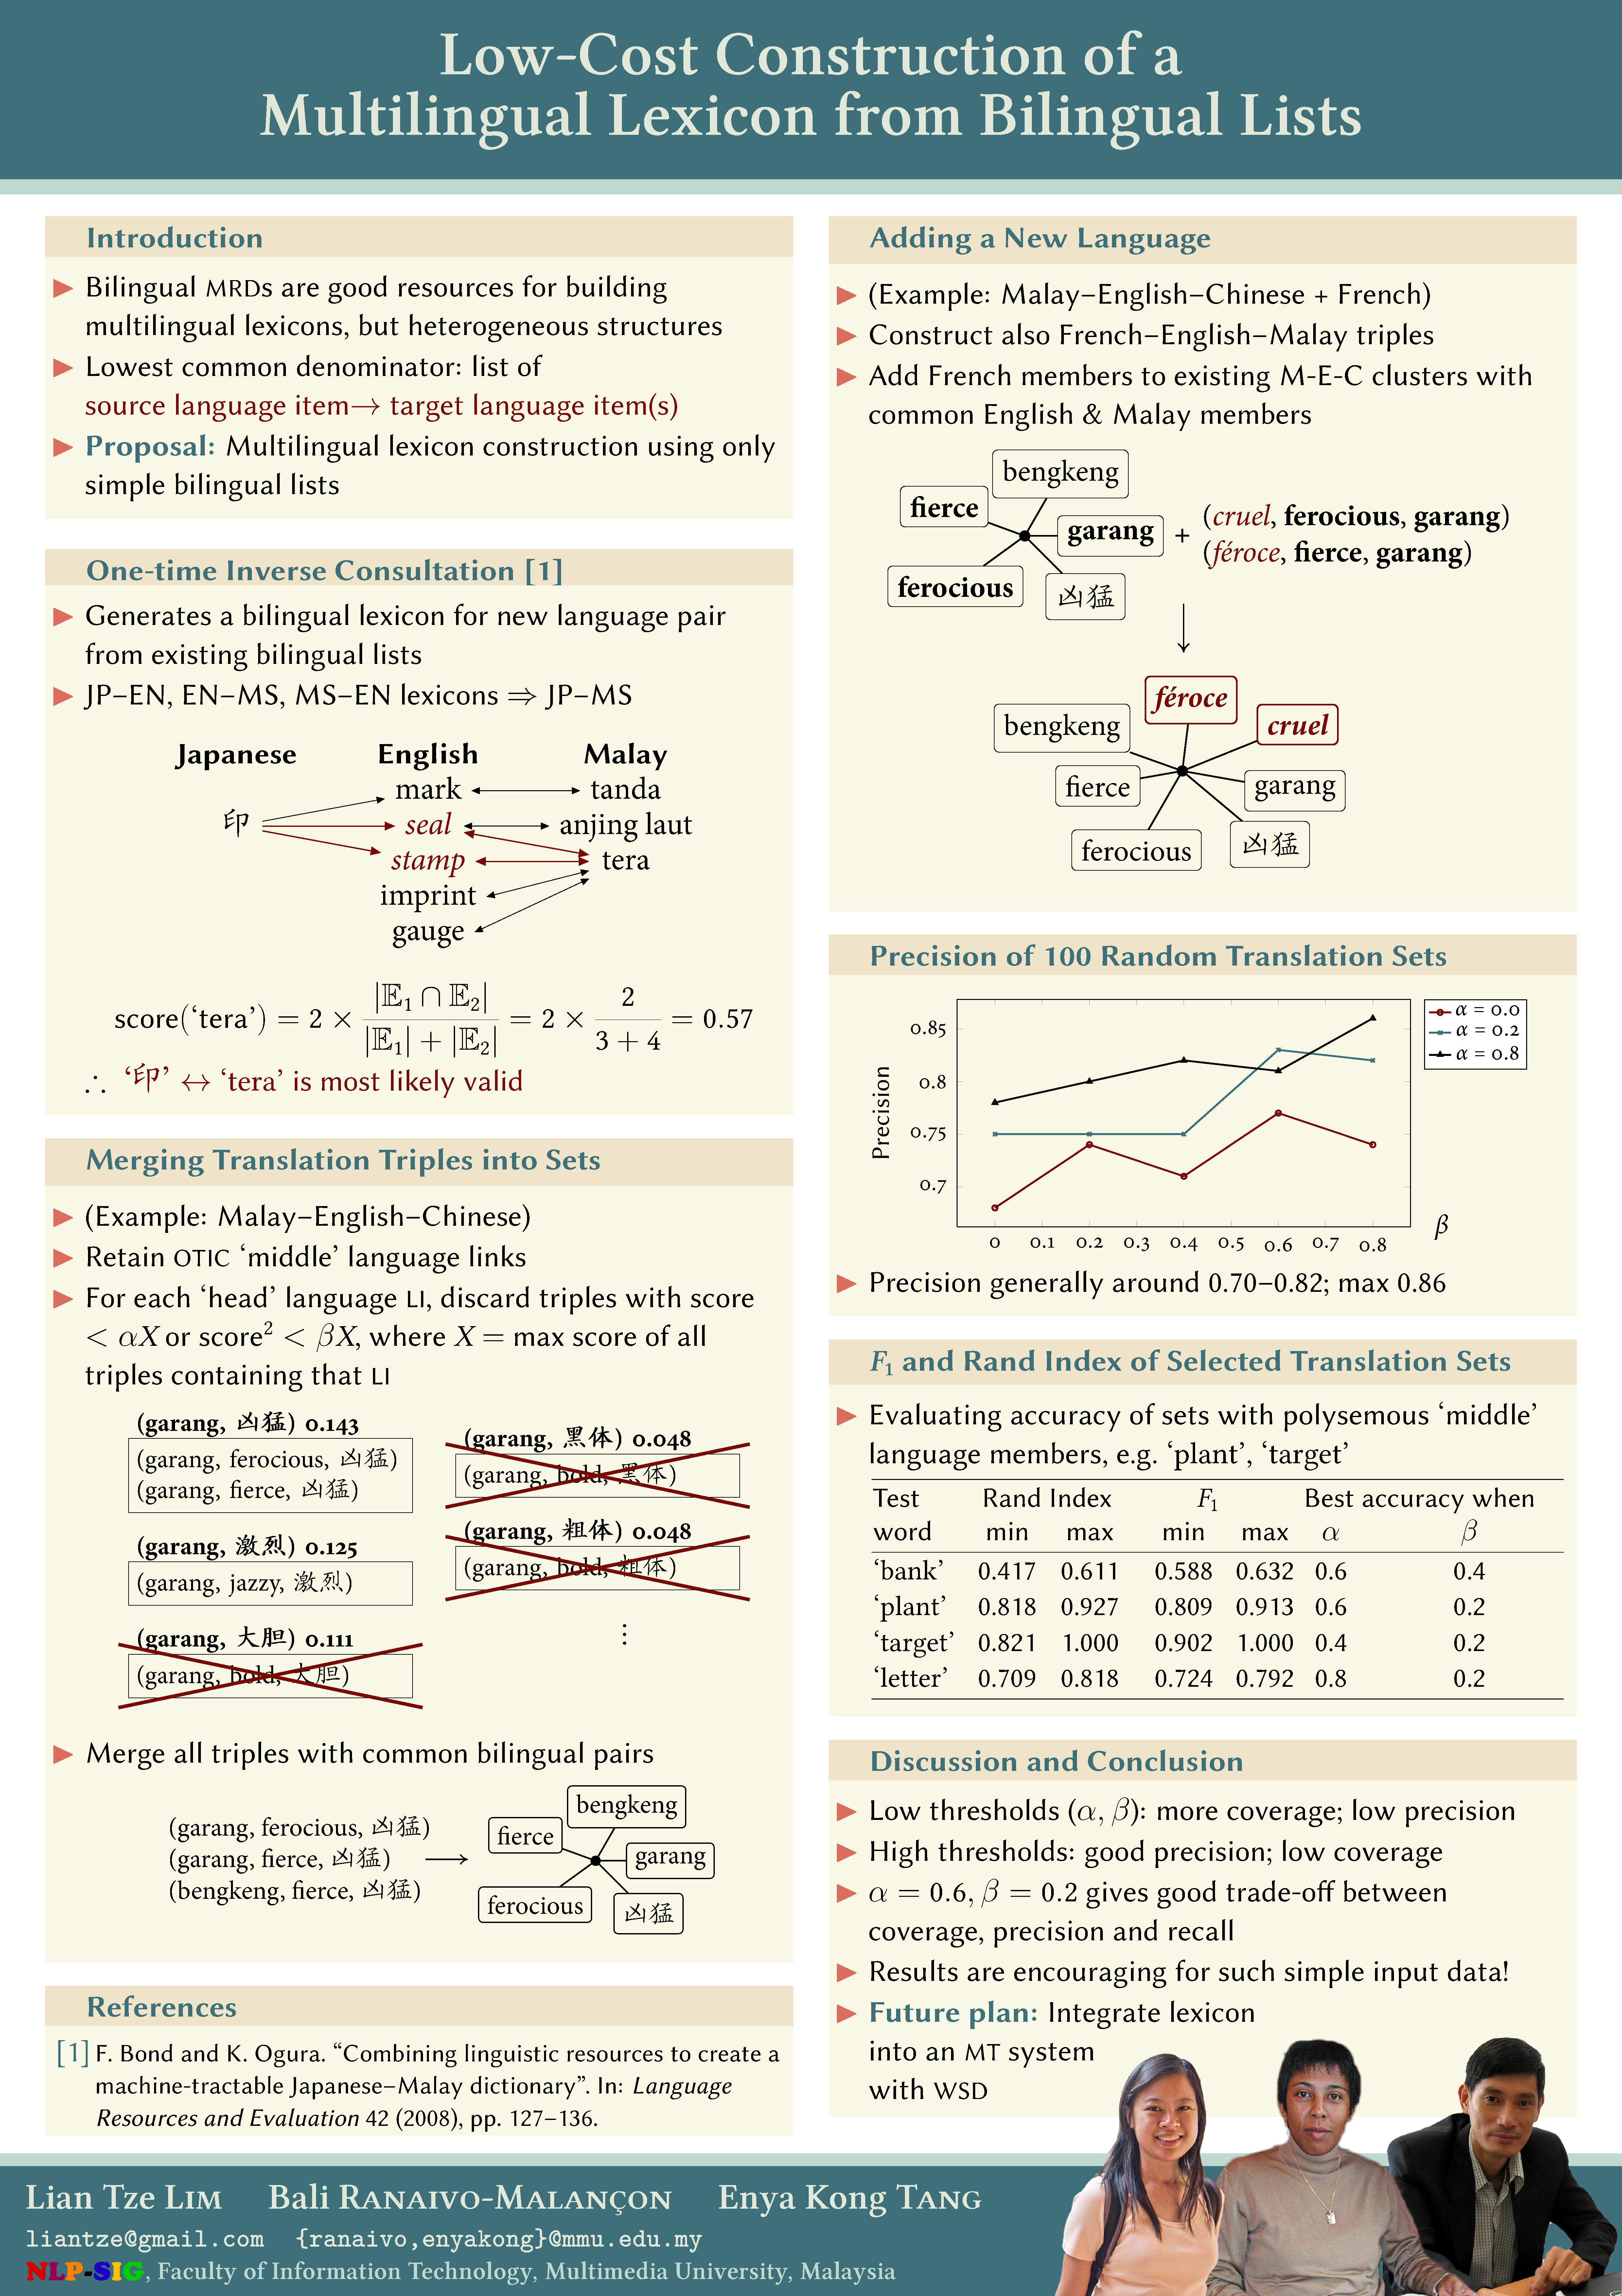
\includegraphics[width=.8\linewidth]{examples/cicling-poster-small.pdf}}}%
\onslide<3|trans:0|handout:0>{\llap{\fcolorbox{black}{white}{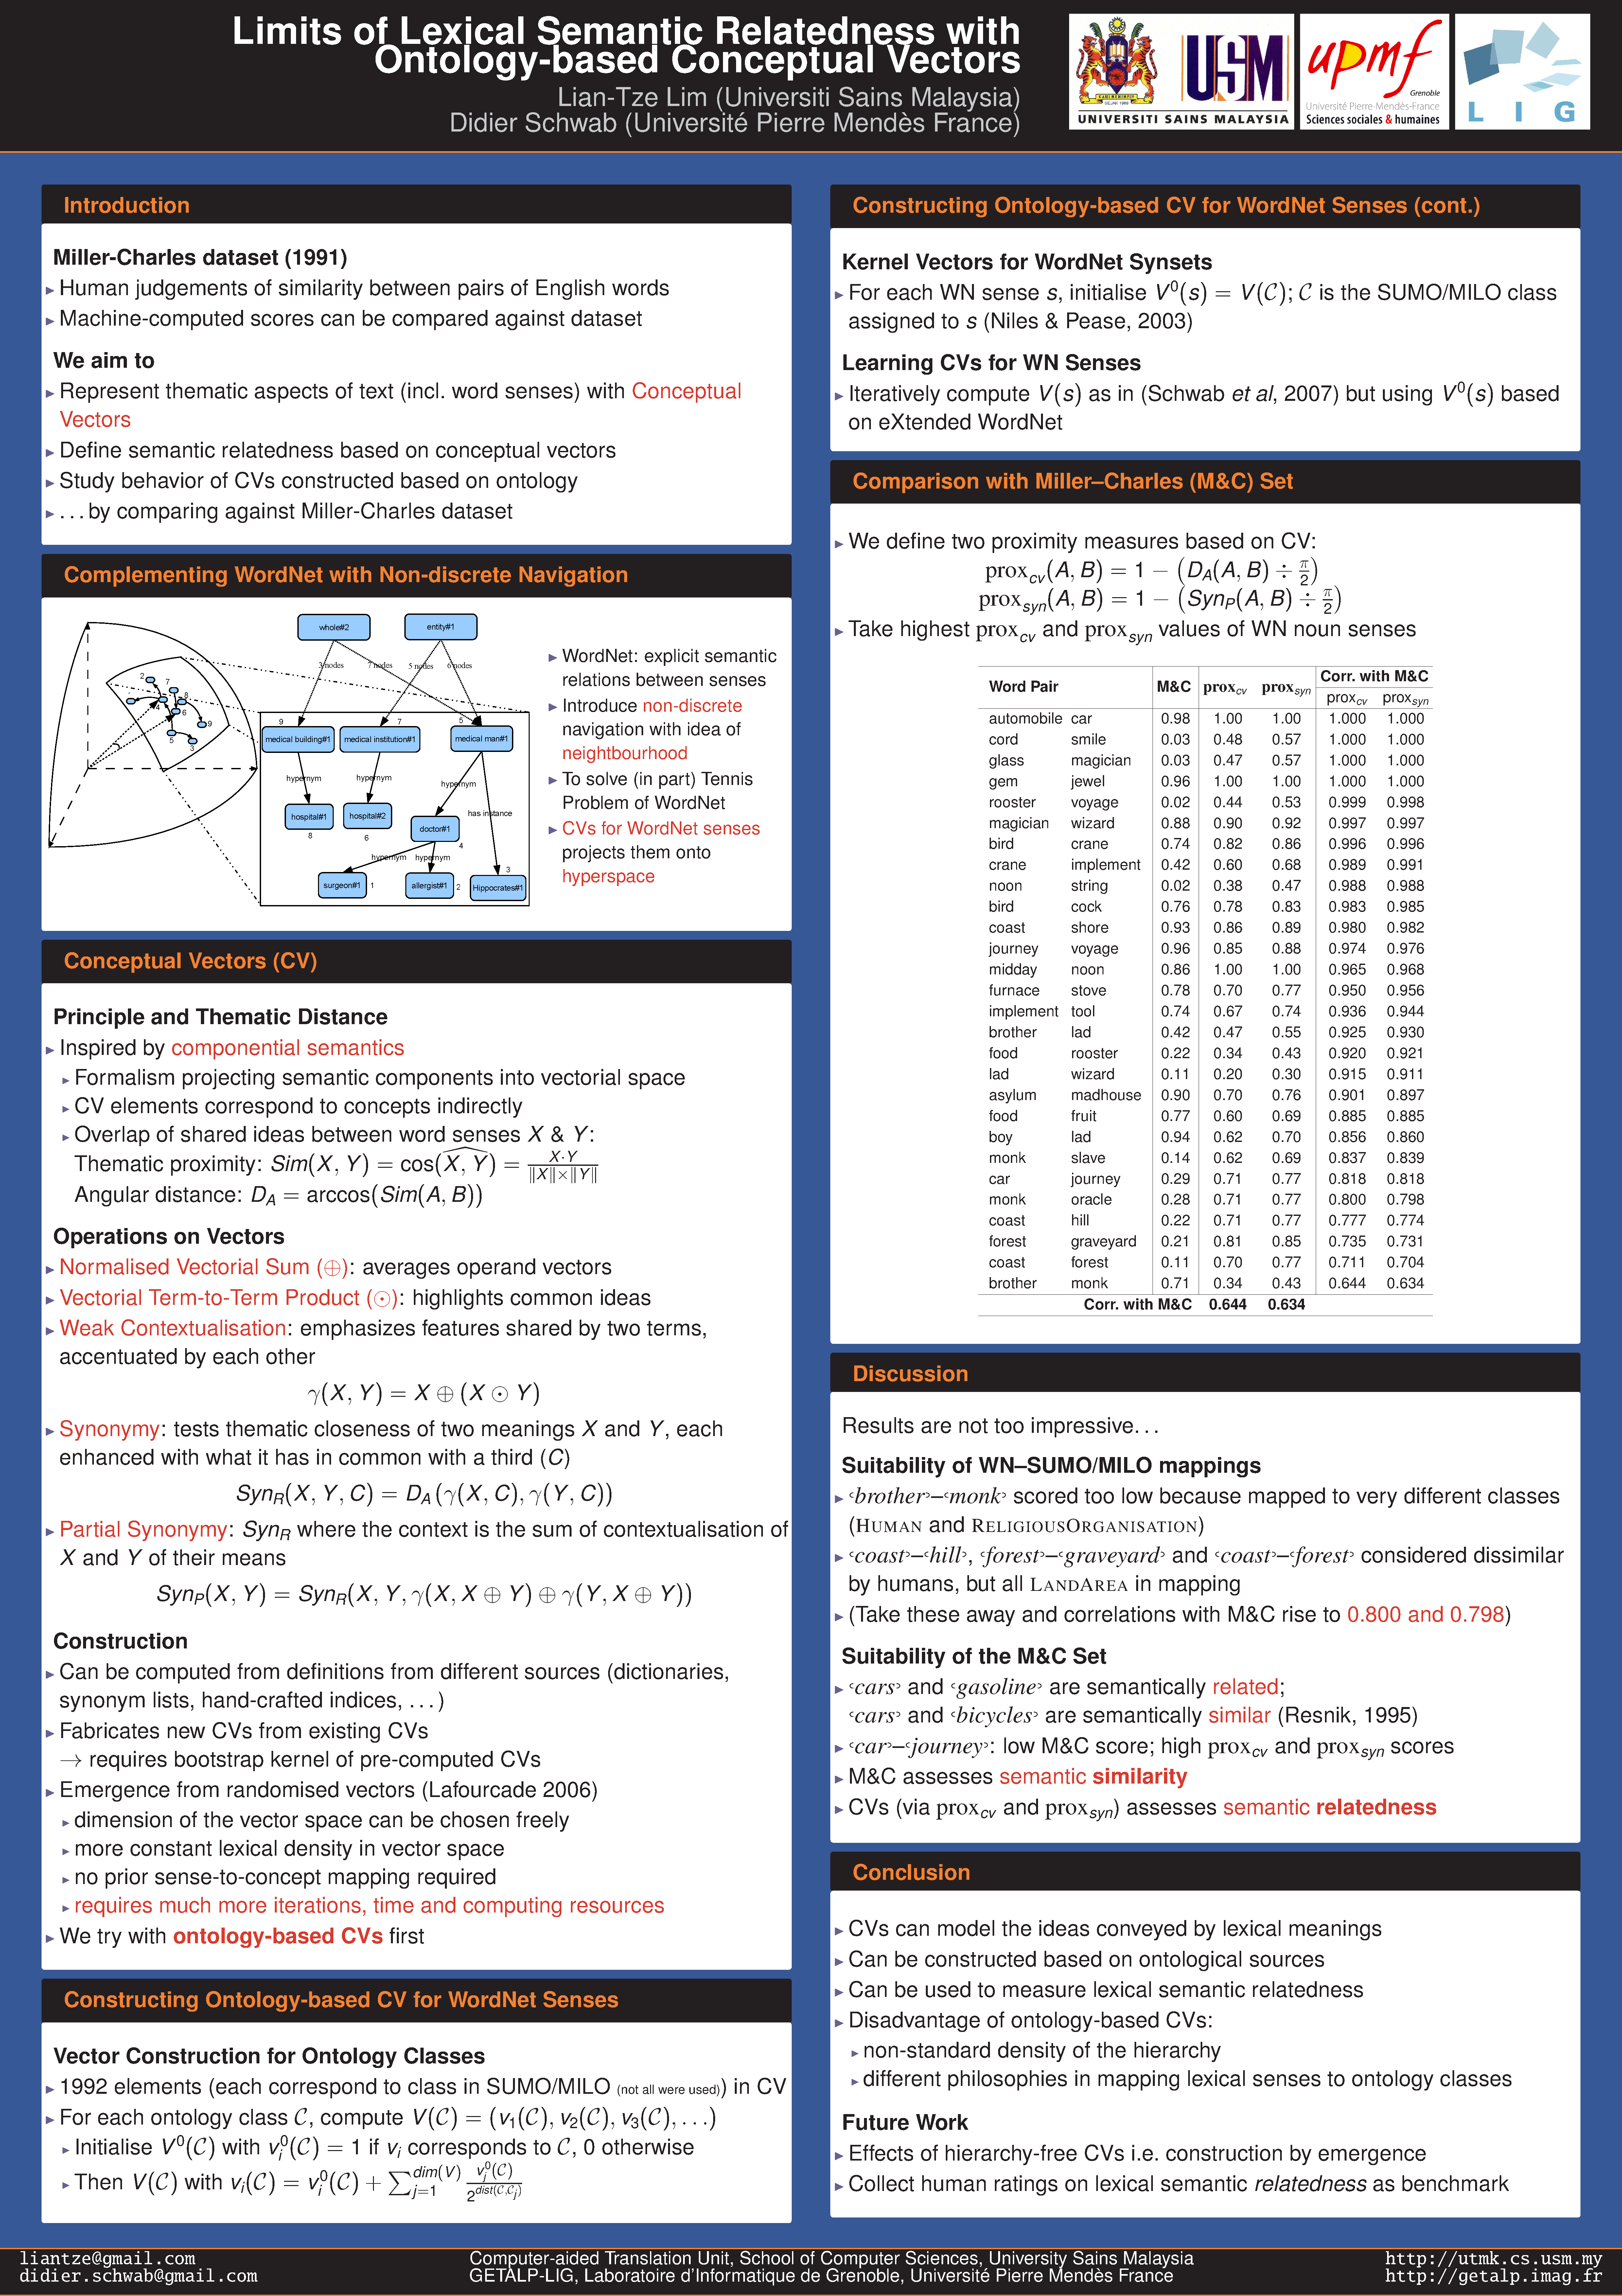
\includegraphics[width=.8\linewidth]{examples/NLPCS08-poster-small}}
}}
\end{column}
\end{columns}

\onslide<4|trans:0|handout:0>{\vspace*{-.75\textheight}}

% tikzposter
\begin{columns}<4|trans:0|handout:0>
\begin{column}{.5\textwidth}
\begin{beamerboxesrounded}[width=\linewidth]{}
\begin{lstlisting}[basicstyle=\ttfamily\small,
moretexcs={usetheme,frametitle,frame},
emph={beamer,beamerposter,frame},
escapechar={:},lineskip=-2pt]
\documentclass[25pt,a1paper]{tikzposter}
\usetheme{Envelope} % nice themes!
\author ... % Meta-information

\begin{document}
... % Poster contents goes here
\end{document}
\end{lstlisting}
\end{beamerboxesrounded}
\end{column}
\begin{column}{.48\textwidth}
\centering
% See http://latex-my.blogspot.com/2011/03/creating-academic-posters-and-printing.html
\onslide<4>{\fcolorbox{black}{white}{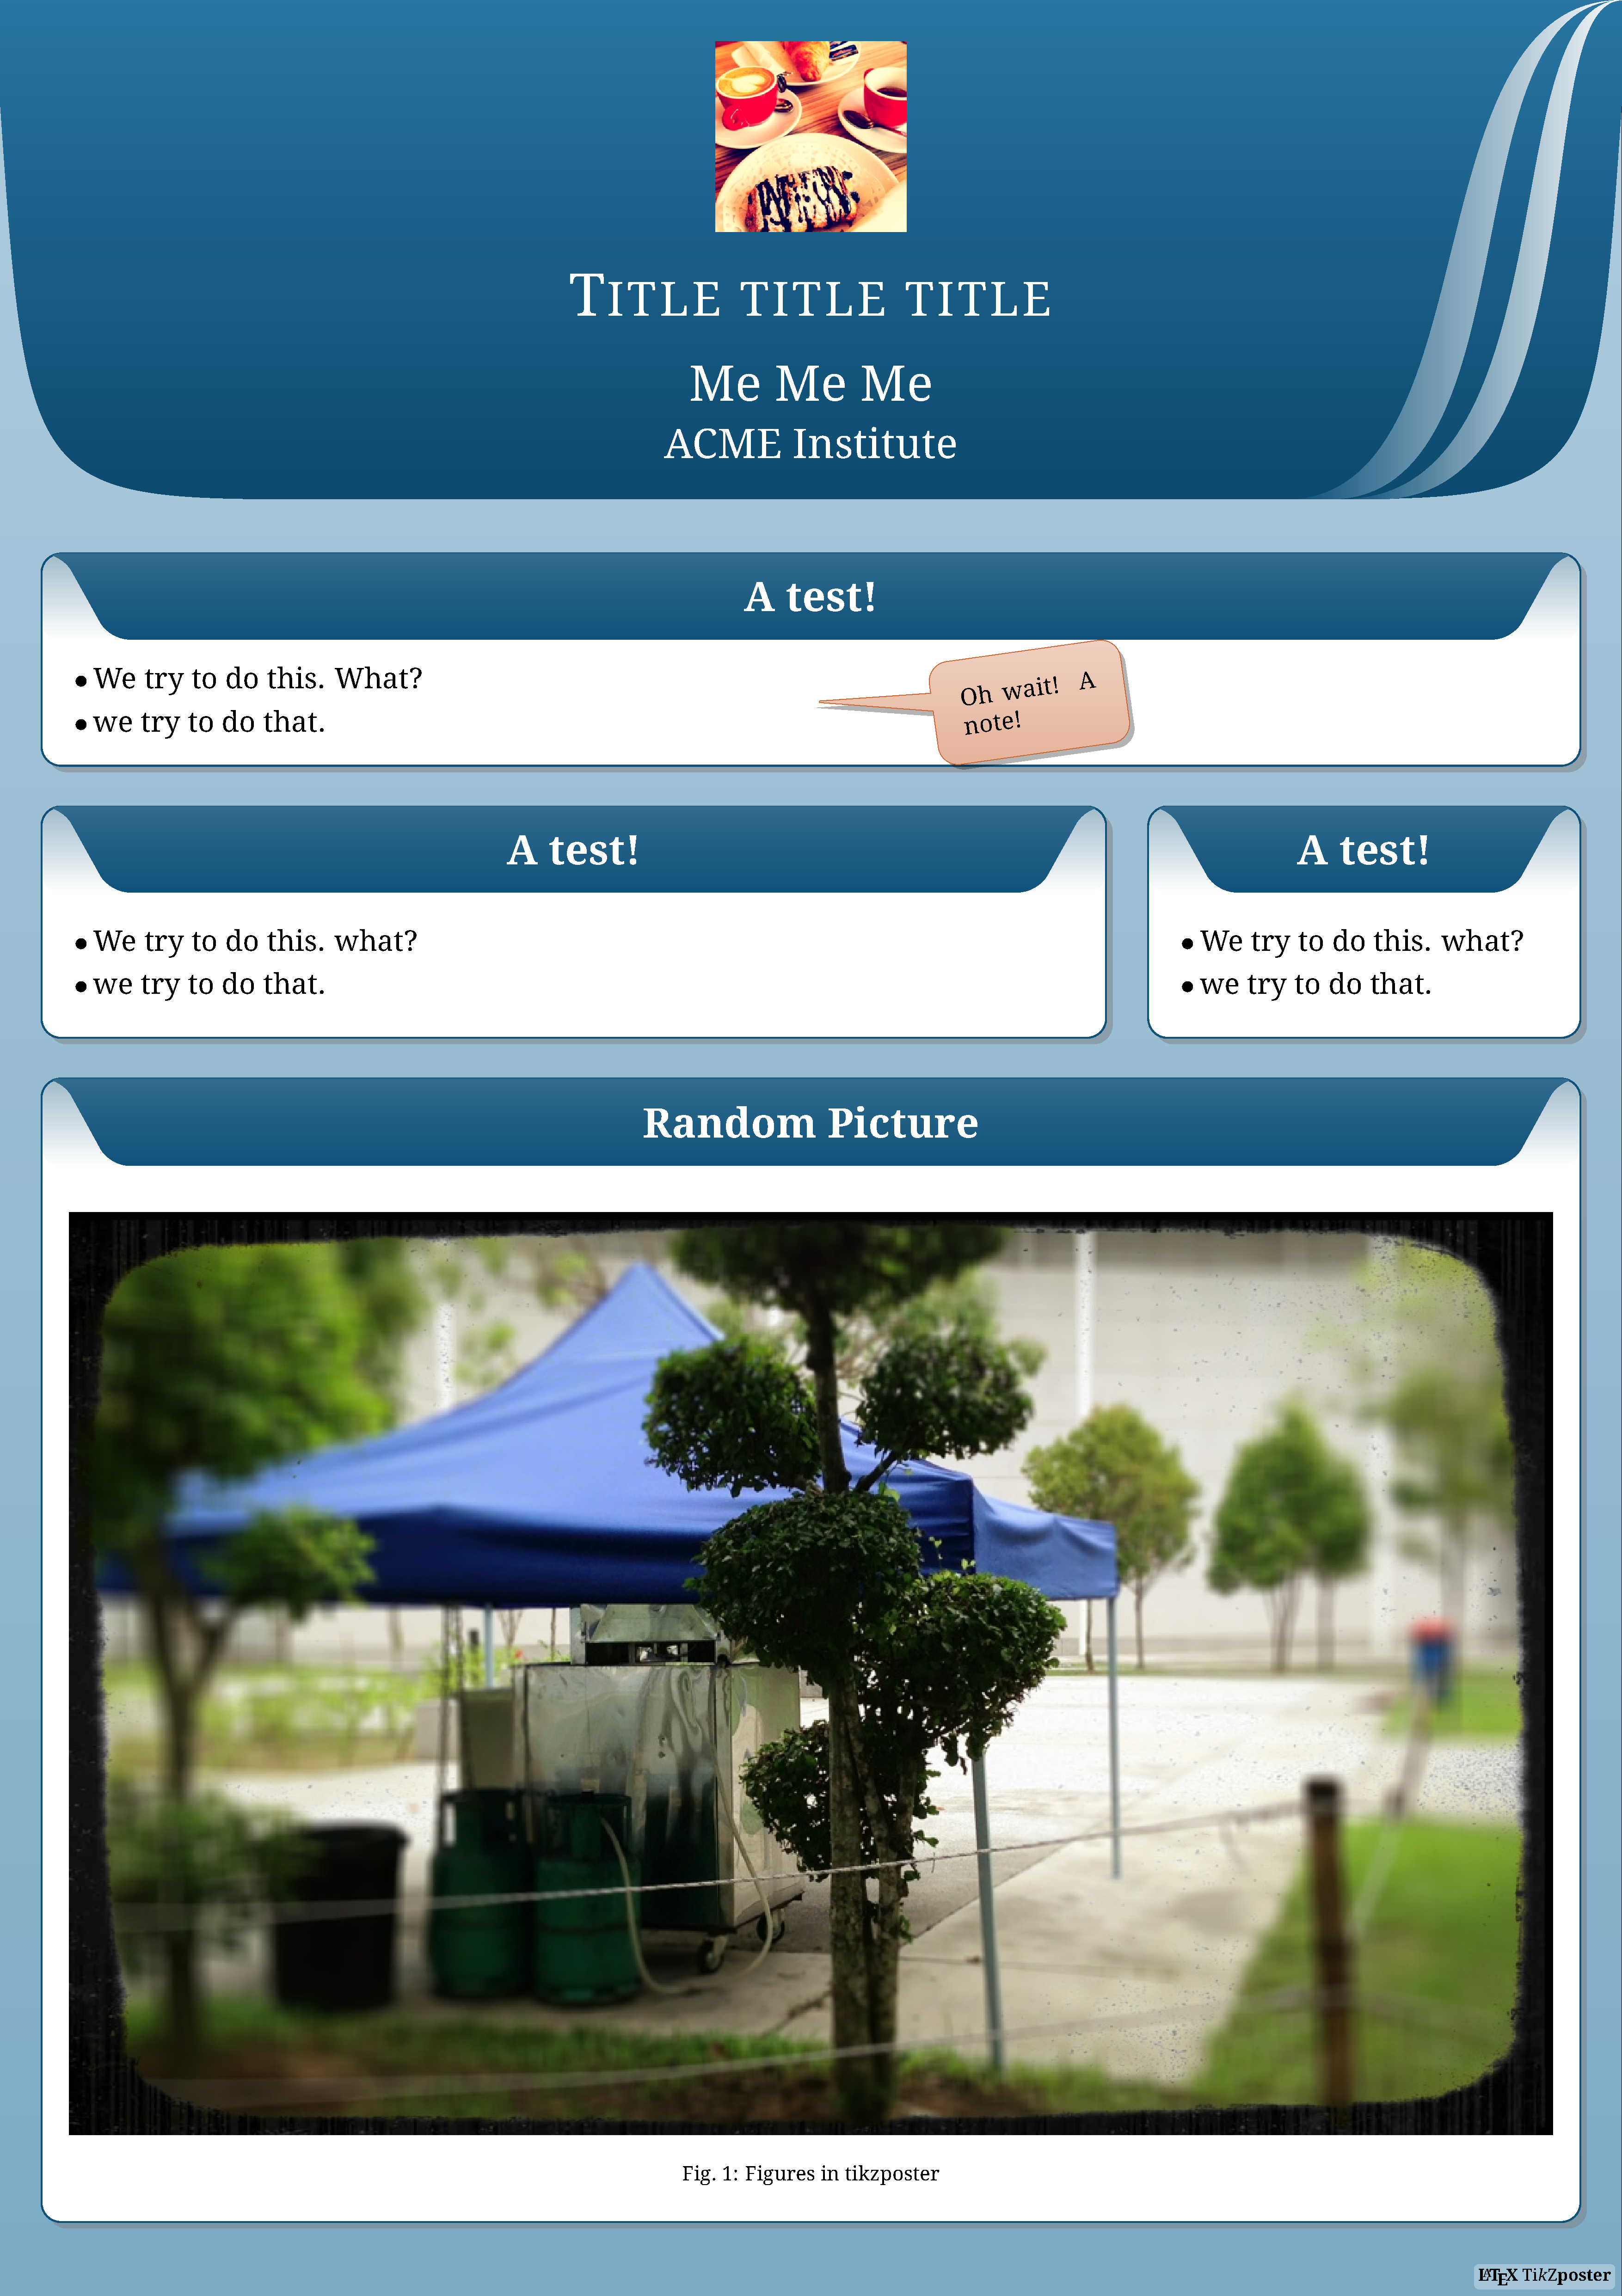
\includegraphics[width=.8\linewidth]{examples/sample-tikzposter.pdf}}}%
\end{column}
\end{columns}

\end{frame}


\begin{frame}[fragile]
\frametitle{Leaflets}

\begin{itemize}
\item \texttt{leaflet}: arrange contents into 6 pages on a foldable double-sided sheet
\end{itemize}

\begin{columns}
\begin{column}{.496\textwidth}
\begin{beamerboxesrounded}[width=\linewidth]{}
\begin{lstlisting}[basicstyle=\ttfamily\small,lineskip=-2pt,emph={leaflet},moretexcs={maketitle}]
\documentclass[foldmark,a4paper]
{leaflet}
\author ... % Meta-information

\begin{document}
\maketitle
\section ...
... % Leaflet contents
\end{document}
\end{lstlisting}
\end{beamerboxesrounded}
\end{column}
\begin{column}{.48\textwidth}
\centering
% See http://latex-my.blogspot.com/2011/04/making-leaflets-with-l-t-e-x.html
\fcolorbox{black}{white}{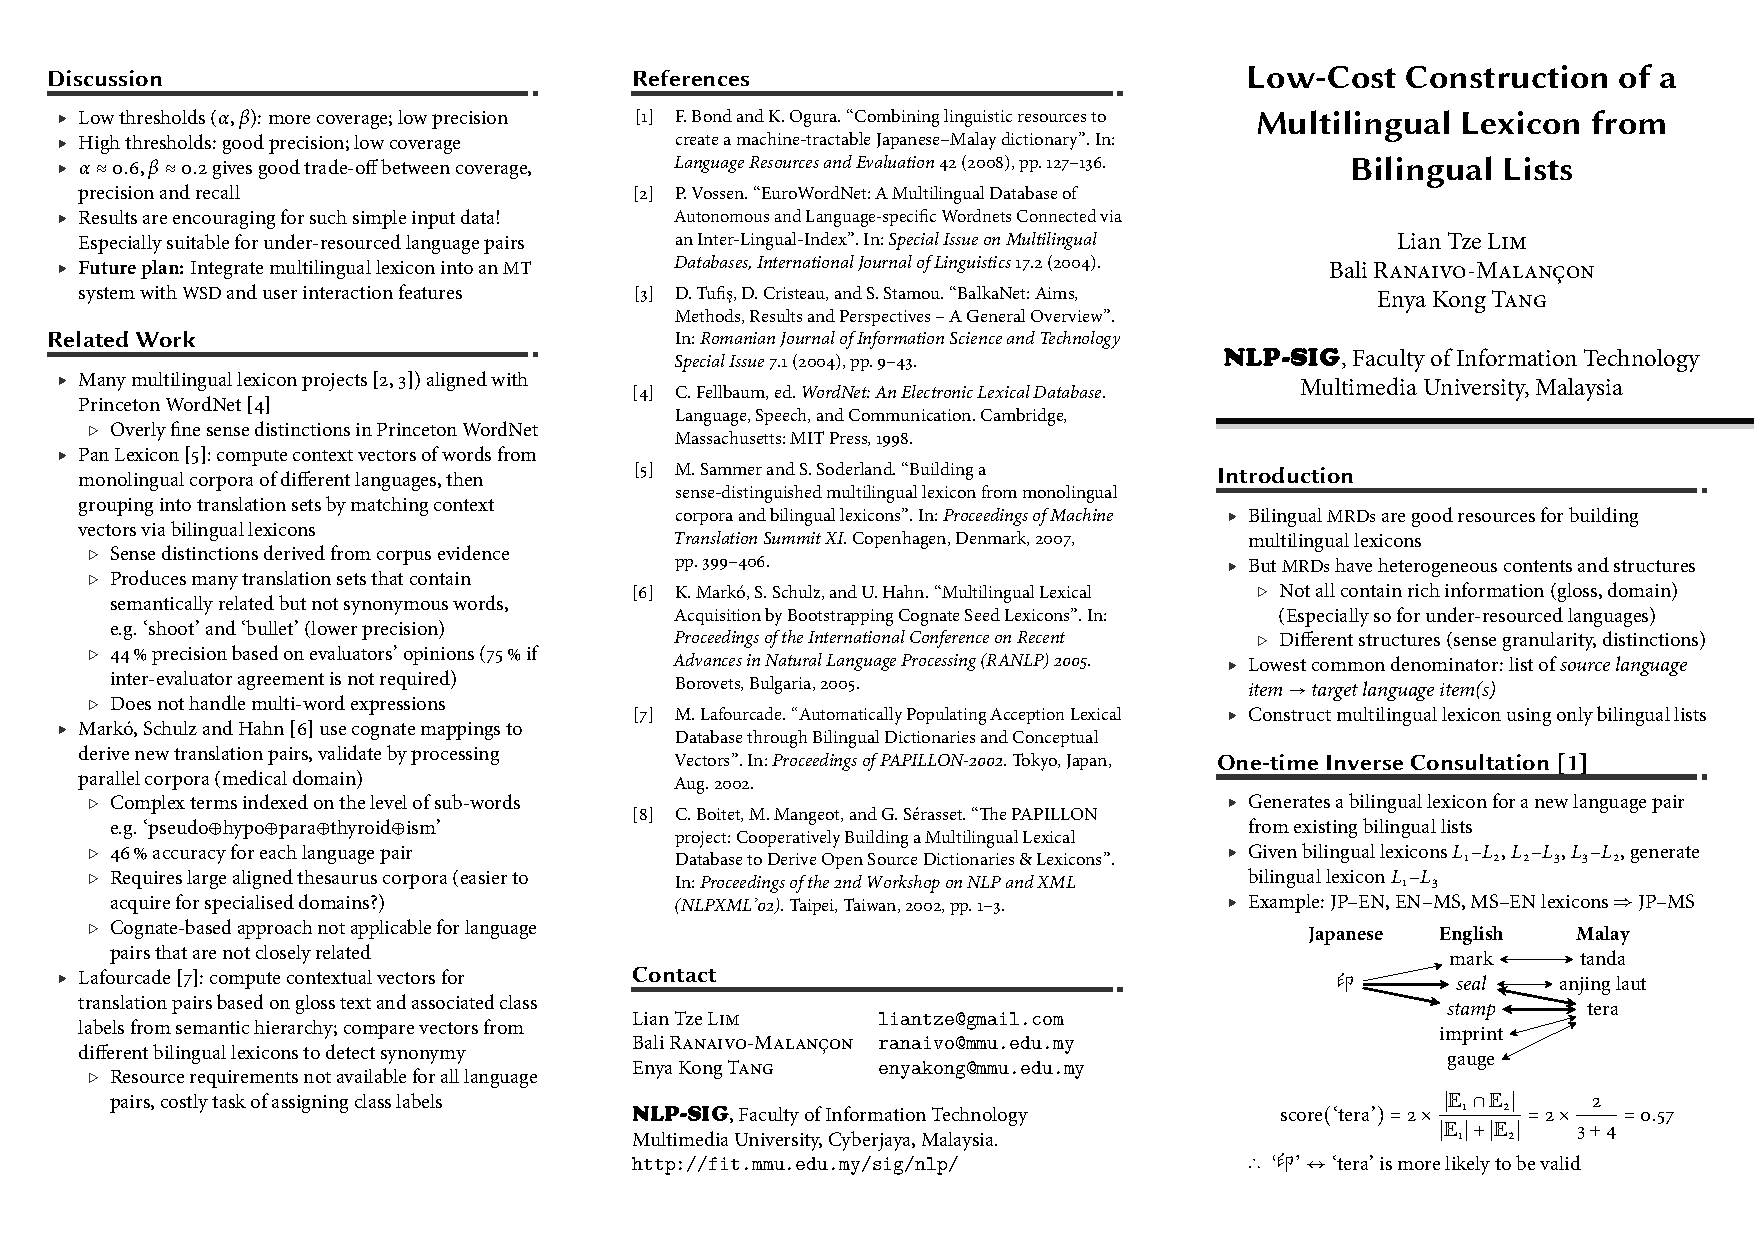
\includegraphics[width=.85\linewidth,page=1]{examples/cicling-handout.pdf}}
\fcolorbox{black}{white}{\includegraphics[width=.85\linewidth,page=2]{examples/cicling-handout.pdf}}\par
\end{column}
\end{columns}

\end{frame}


\begin{frame}[fragile,allowframebreaks]
\frametitle{Fillable \textsmaller{PDF} Forms}
\begin{columns}
\begin{column}{.52\textwidth}
\begin{beamerboxesrounded}{}
\begin{lstlisting}[basicstyle=\ttfamily\small,escapechar=|,
moretexcs={TextField,ChoiceMenu,CheckBox},
emph={hyperref}]
\usepackage{hyperref}
... % various settings skipped
\TextField{Name:}\\
\TextField{Affiliation:}\\
\ChoiceMenu[radio=true]
{Are you a:}{Student, Academic}\\
Interest:
\CheckBox{Security}
\CheckBox{Systems}
\CheckBox{User space}\\
\TextField[multiline=true]
{Comments:}\\
\end{lstlisting}
\end{beamerboxesrounded}
\end{column}
\begin{column}{.47\textwidth}
\centering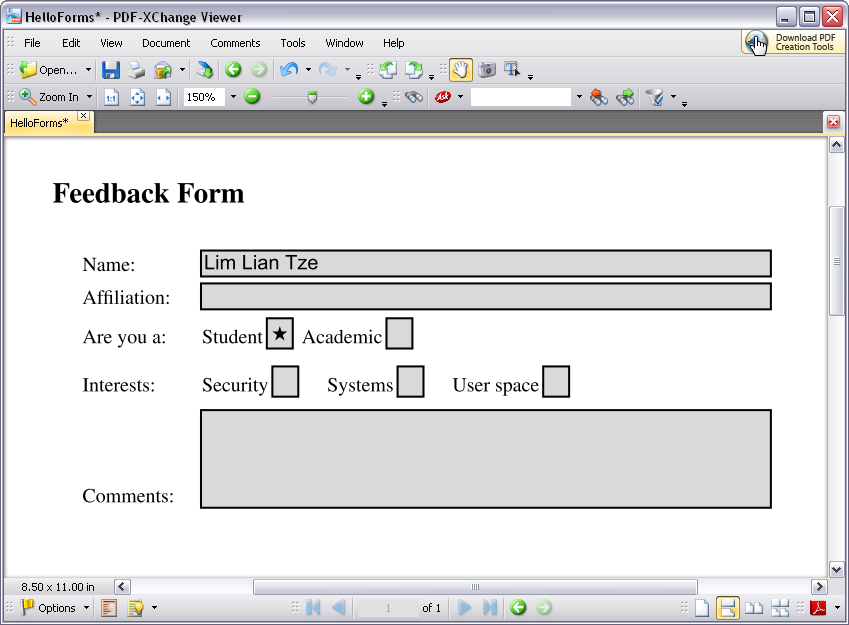
\includegraphics[width=\linewidth]{examples/form-screencap}\par
\end{column}
\end{columns}
\pagebreak

\alert{Use with caution!}
\begin{itemize}
\item \texttt{poppler}-based viewers (\texttt{evince}, \texttt{xpdf}, \texttt{okular})
\begin{itemize}
\item Problem displaying and saving radio/check boxes correctly
\item Saved forms can't be opened by other viewers
\end{itemize}
\item Adobe Reader
\begin{itemize}
\item Cannot save filled form as \textsmaller{PDF} unless Acrobat is installed
\item Only as field-and-value text file
\item Can provide ``Submit'' button for submission to a \textsmaller{URL}
\item Or print hard copy of filled form!
\end{itemize}
\item PDF XChange Viewer
\begin{itemize}
\item Best freeware for filling and saving \LaTeX-created forms
\item Windows only
\item Not \textsmaller{OSS}
\end{itemize}
\end{itemize}

\end{frame}


\begin{frame}[fragile]
\frametitle{Flash Cards}
\begin{columns}
\begin{column}{.465\textwidth}
\begin{beamerboxesrounded}{}
\vskip-1em
\begin{lstlisting}[basicstyle={\ttfamily\small},
emph={flashcards,flashcard},
moretexcs={cardfrontstyle,cardfrontfoot}]
\documentclass[avery5388,frame]
{flashcards}
\cardfrontstyle{headings}
\cardfrontfoot{Linux}

\begin{document}
\begin{flashcard}[Security]
{Certificate}
...
\end{flashcard}

\begin{flashcard}[Security]
{MAC ...}
...
\end{flashcard}
\end{document}
\end{lstlisting}
\vspace*{-1em}
\end{beamerboxesrounded}
\end{column}

\begin{column}{.53\textwidth}
\centering

\includegraphics[width=.49\linewidth,page=1]{examples/flashcard-crop}\hfill
\includegraphics[width=.49\linewidth,page=2]{examples/flashcard-crop}
\par
\end{column}
\end{columns}
\end{frame}


\begin{frame}[fragile]
\frametitle{Examination Paper}
\begin{columns}[T]
\begin{column}{.49\textwidth}
\begin{beamerboxesrounded}{}
\vskip-1em
\begin{lstlisting}[moretexcs={question,choice,CorrectChoice,part,printanswers},
emph={exam,questions,oneparchoices,parts,solution},
basicstyle=\ttfamily\scriptsize\lsstyle,lineskip=-1pt,escapechar=;]
\documentclass{exam}
...
\begin{questions};\onslide<2>{\bfseries\color{Maroon}\textbackslash printanswers};
\question[5] 
What is Paul McCartney's middle name?
\begin{oneparchoices}
\choice John \CorrectChoice Paul 
\choice Ringo \choice James
\end{oneparchoices}

\question[10] What was the Beatles' first single in 1962?
\begin{solution}Love Me Do\end{solution}

\question
\begin{parts} 
\part[5] What was George's inspiration for `While My Guitar Gently Weeps'?
\begin{solution}
He opened a random book and saw the words ``gently weep''.
\end{solution} 
...
\end{questions}
\end{lstlisting}
\vspace{-1em}
\end{beamerboxesrounded}
\end{column}
\begin{column}{.49\textwidth}
\centering
\onslide<1|trans:0|handout:0>{\fcolorbox{black}{white}{\includegraphics[width=\linewidth,page=1]{examples/exam}}}%
\onslide<2>{\llap{\fcolorbox{black}{white}{\includegraphics[width=\linewidth,page=2]{examples/exam}}}}
\end{column}
\end{columns}
\end{frame}

% \begin{frame}[fragile]
% \frametitle{KDU-exam}
% \begin{itemize}
% \item Automatic cover generation
% \item Automatic calculation of section marks, total marks, number of sections, number of pages
% \item Takes care of all formattings
% \end{itemize}

% \vspace*{-\baselineskip}
% \begin{columns}
% \begin{column}{.47\textwidth}
% \begin{beamerboxesrounded}{}
% \vskip-1em
% \begin{lstlisting}[moretexcs={coversubj,semester,examsection,droppoints,sectionpoints}]
% \coversubj{DIT1234 A Cool Subject}
% \semester{August 2013}
% ...

% \examsection{Basic Concepts}
% \begin{Questions}
% \Q[5] Give 5 examples. \droppoints
% \Q[8] Explain 4 concepts. \droppoints
% \end{Questions}
% \sectionpoints
% \end{lstlisting}
% \vspace{-1em}
% \end{beamerboxesrounded}
% \end{column}
% \begin{column}{.5\textwidth}
% \onslide<2>{\fcolorbox{black}{white}{\includegraphics[page=1,width=.8\textwidth]{sample}}}
% \onslide<3>{\llap{\fcolorbox{black}{white}{\includegraphics[page=2,width=.8\textwidth]{sample}}}}
% \end{column}
% \end{columns}

% \end{frame}